\documentclass[twocolumn]{article}
%\documentclass[authoryear, 12pt,5p, times]{elsarticle}
%\usepackage[hypcap]{caption}
%\geometry{margin=0.95in,top=1.4in,bottom=1.4in}
%\geometry{margin=1.1in,top=1.5in,bottom=1.5in}
%\textwidth=5cm
\usepackage{enumitem}
\usepackage{graphicx}
\usepackage{float}
\usepackage{amsmath}
\usepackage[hidelinks]{hyperref} 
 \usepackage{gensymb}
\usepackage{subcaption}
\usepackage{url}
%\renewcommand\thefootnote{\fnsymbol{\dagger}}
\usepackage[symbol*]{footmisc}
\makeatletter
\newcommand{\rpm}{\raisebox{.3ex}{$\scriptstyle\pm$}}
\begin{document}
%\begin{frontmatter}
%a)              A title page with your name, your partner’s name, the date, and a short abstract (less than 100 words) summarizing your circuit and the results of any measurements.
\title{Final Project: Optical Theremin}\vspace{-20pt}
\author{\today \quad \\Jung Lin (Doris) Lee [Lab Partner: Leah Tom]\\Prof. William Holzapfel, GSI Thomas Darlington, Thomas Mittiga, John Groh,  \\Victoria Xu, Jonathan Ma, Francisco Monsalve, Xiaofei Zhou\vspace{-20pt}}	 
\date{}
\maketitle
\begin{abstract}
Applying our knowledge about op-amps, transistors, diodes and knowledge from the previous labs, we designed and built an optical theremin that changes the frequency and amplitude of the sound output based on the amount of light incident on the device. The circuit consists of bandpass filter, full wave rectifier, voltage-controlled oscillator, and relaxation oscillator module that are connected in series to perform the modulation. With various circuit modifications described in this report, we improved the performance of the modulation control, attaining a distinctly audible dynamic range of 5V and frequency range of 1 octave. %ahat we implemented and demonstrate how they improved the performance of the modulation control and the audio quality of the theremin.  % In this report, we describe the reasoning behind the 
 \end{abstract}
\section{Introduction}
%b)              A one-page introduction.
 gained popularity in media ,
Theremins named ---, Its characteristic eerily-sounding tunes are often featured on movie soundtracks and pop and rock music after Leon Theremin invented the device in the 1920s. Most existing implementations of theremin consist of two metal antennas operating at radio frequencies. The performer's hand acts as a variable capacitor determining the frequency of the oscillator circuit changes the distance between the antennas and the grounded plate, between , thereby controlling the volume and pitch of the output sounds.
\par Our project was initially inspired by  Bonnie Eisenman's \textit{Illumaphone} project {\footnotesize[7]}, optical theremin piano with 6 light ---- cups.  Most DIY optical theremin projects contains relatively simply circuitry of only a single photoresistor whose output is fed to a microcontroller  the hassle of doing signal processing and filtering on the hardware level and leaving most of the work to the music processing software. We distinguish our project from these prior works by designing a optical theremin that takes an entirely hardware-based approach to encompasses all the signal acquisition, filtering, processing, and audio output steps. 
\par Our design concept motivated us to include noise-reducing modules such as the bandpass filters, synced with the relaxation oscillator's output frequency. Challenging task of achieving audible sounds, were  carefully designed and ----- inverting amplifiers. Although we are unable to achieve as much as the dynamic range and smooth sound quality as the \textit{Illumaphone} with this entirely hardware-based approach, we have ---- sufficiently --- our design objectives for this project.
\section{Circuit Description}
c)               A description of your circuit:
\subsection{Functional Description}
i)                Start with a functional description: a block diagram listing all the major operations in your circuit.
\begin{figure*}
 \centering
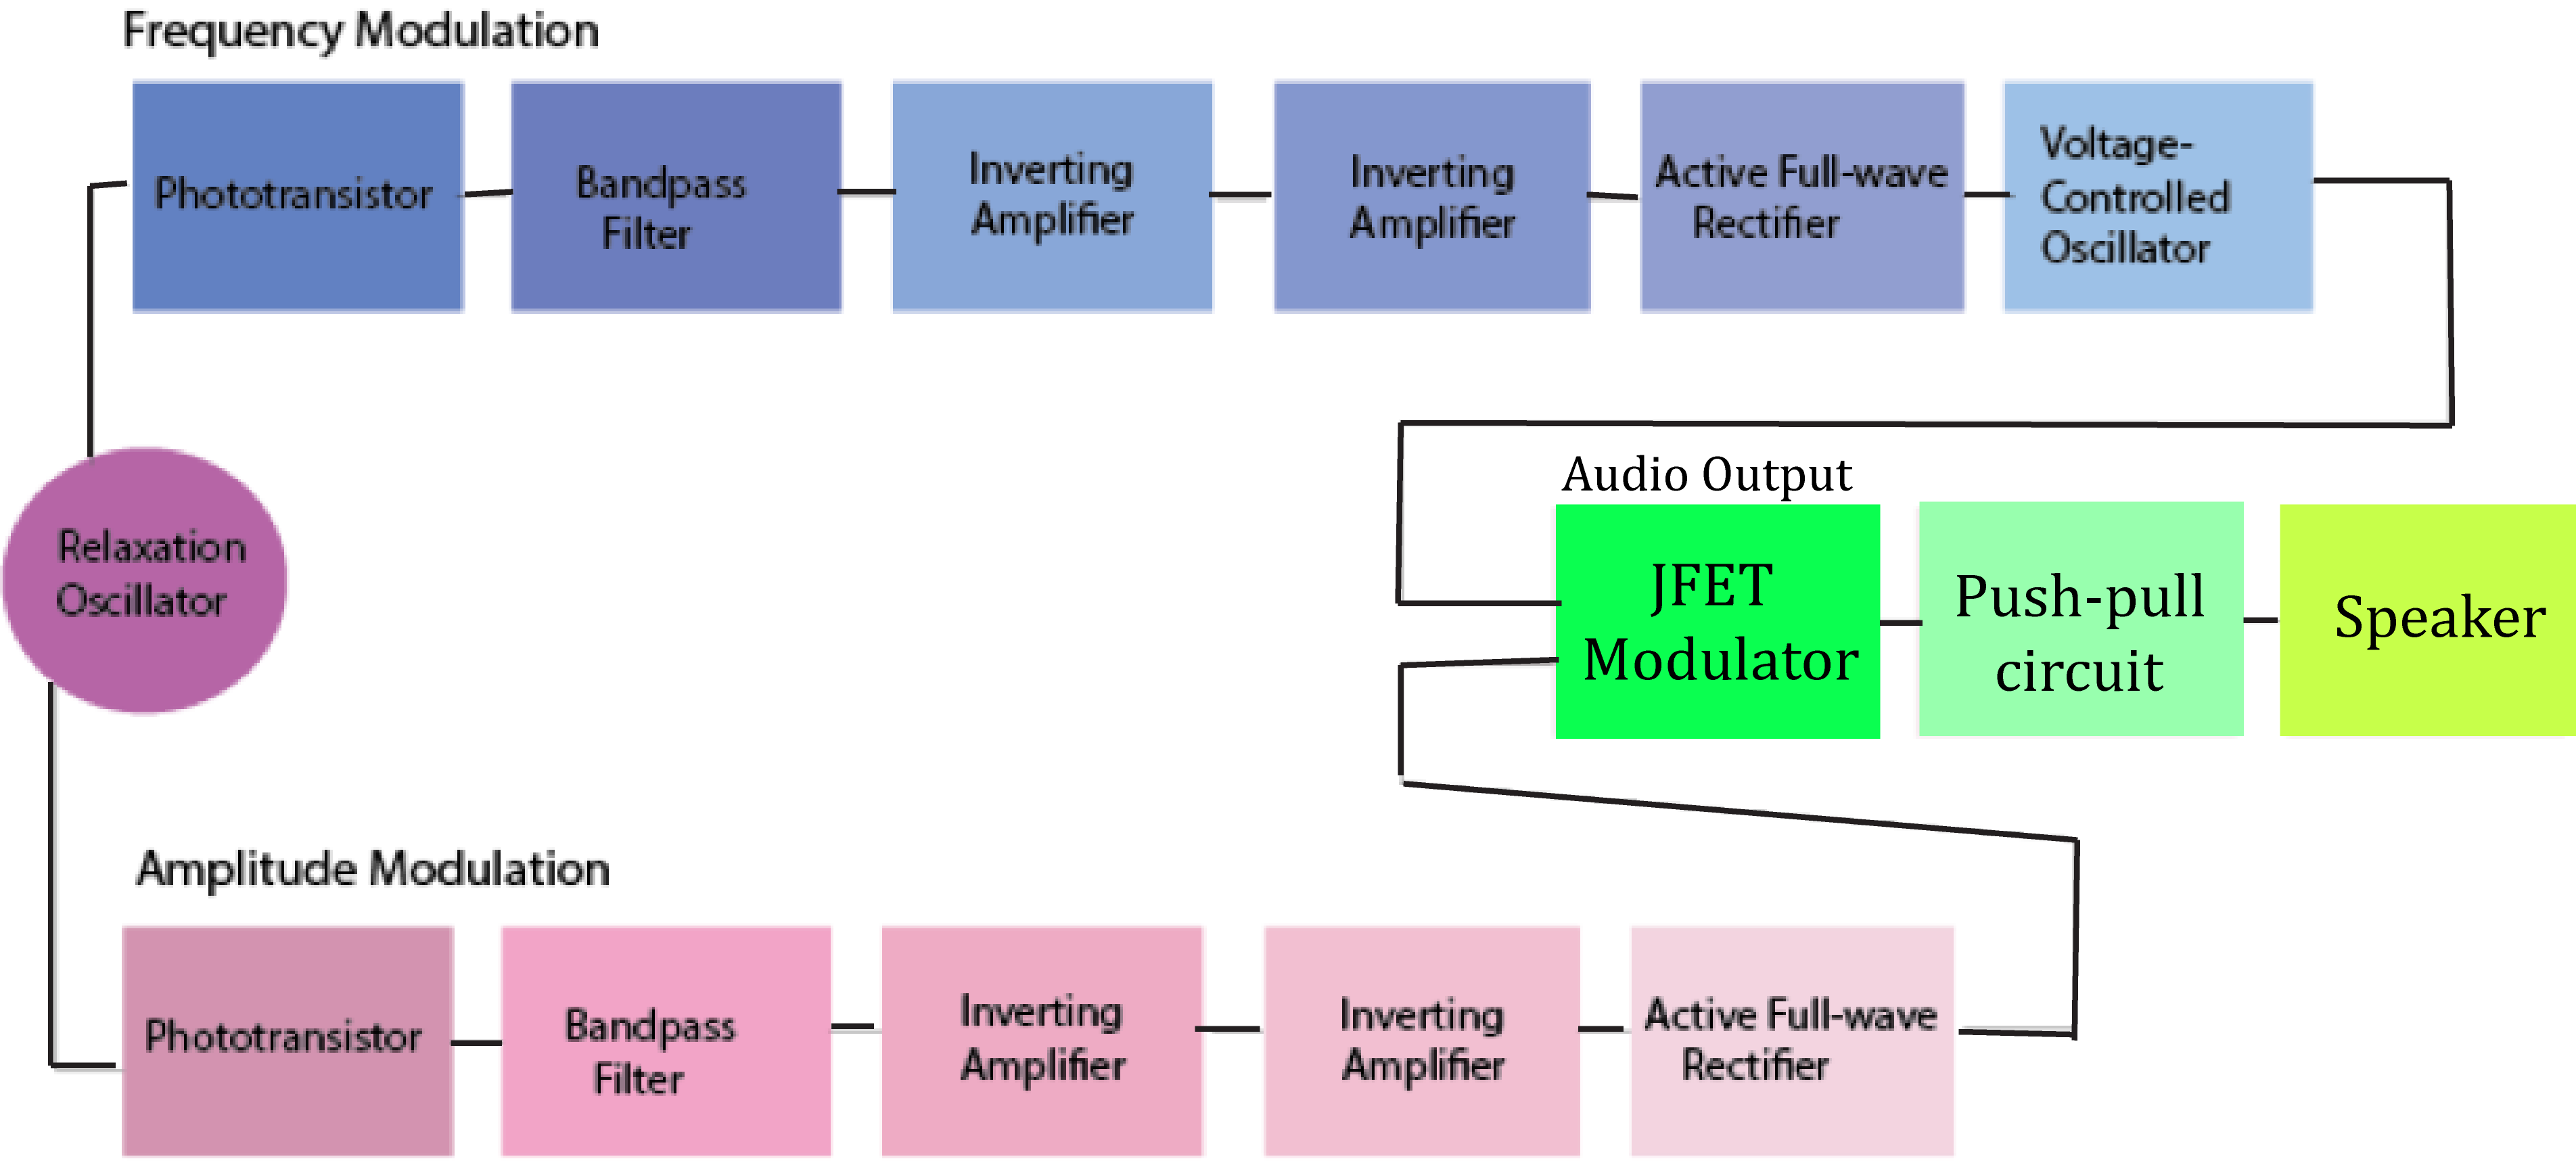
\includegraphics[width=450pt]{figure/block}
\caption{Block diagram of circuit modules. Green denotes modules responsible for audio output. The red and blue denotes modules responsible for amplitude and frequency modulation respectively.}
\label{block}
\end{figure*}
ii)              A readable circuit diagram.
\subsection{Component Description}
%iii) A description of the purpose and operation of all the major components in the circuit (most likely all the active components and some of the passive components.)  Relate each major component to the appropriate function block.
\subsubsection{Bandpass filters}
Initially, the filters was designed to pass through signals of frequencies between 900 and 1100 Hz. Using a 1$\mu$F capacitor, we computed the resistance values as: 
\begin{align*}
f = \frac{1}{2\pi RC}
\\ R = \frac{1}{2\pi (1.0\times10^{-6} F)f}
\end{align*}
Since we found that the signal that passes through was too low, we redesigned a the filters to increase the range to 500$\sim$2000 Hz.
\subsubsection{Inverting Amplifer}
\par We also build two inverting amplifier 
We built an inverting amplifier as shown in Fig.\ref{inverting_amp}. First tried using R1= 47k$\Omega$ resistor as we did in the circuit in Lab 6, but we found that since to the variable resistance shown in Table \ref{photor} , the $V_{out}$ only rails as we cover up the photoresistor. In order to map out a more detectable change, we increase the gain by decreasing the value of R1 to 1k$\Omega$, since
\begin{equation}
V_{out} = -R_2I = \frac{-R_2V_{in}}{R_1}
\end{equation}
where the gain is -R2/R1. When testing, we use two 1$\mu$F capacitor to decouple the power supply and minimize the parasitic oscillation. 

\subsubsection{Full Wave Rectifier}
We build a Graetz bridge full wave rectifier using four 1N4007 diodes. Since the diode only passes through current in one direction, the arrangements of diodes shown in Fig.\ref{rectifier}, passes through the positive current and flips the negative signal up.
\begin{figure}[h!]
 \centering
 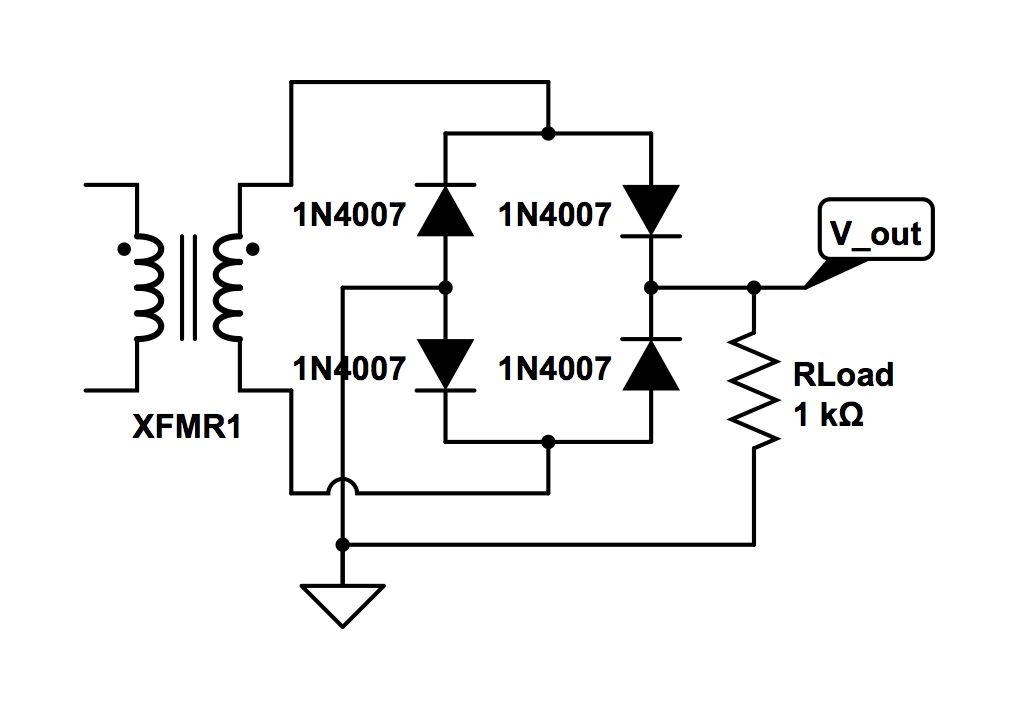
\includegraphics[width=220pt]{figure/full_wave_rectifier.jpg}
\caption{Full Wave Rectifier Circuit.}
\label{rectifier}
\end{figure}
\par The performance of the full wave rectifier is liekley the source of sound quality degradtion in our circuit because -----. Therefore, we used an active full wave rectifier to ----.
\subsubsection{Voltage Controlled Oscillator}
The Voltage Controller 
\subsubsection{JFET Modulator}
Multiplier
\subsubsection{Relaxation Oscillator}
We use a relaxation oscillator to generate the ``On-Off signal" for the LED flashing at 1kHz.
\begin{figure}[h!]
 \centering
 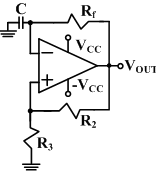
\includegraphics[width=0.2220pt]{figure/relax_osc.png}
\caption{Relaxation Oscillator Schematic.}
\label{relax_osc}
\end{figure}
The output frequency of the circuit is described by :
\begin{equation}
f=\frac{1}{2 R_f C ln\frac{1+\beta}{1-\beta}}
\end{equation}
where $\beta$ is the ratio of the resistances $\frac{R_3}{R_3+R_2}$.
\par Initially, we built the circuit using the combination of $R_f$ = 100$\Omega$ and $R_3 = 100\Omega$, C=1000$\mu$F and $R_2 = 3 M\Omega$. However, we found that the output frequency deviate largely from our computed frequency of 10Hz (initially designed for the photoresistor circuit). We suspect that this is due to our use of a the large 1000$\mu$F electrolytic capacitor. After trying different combinations of resistances and capacitance, we found that the circuit yields optimal performance when $R_2$ and $R_3$ are approximately equal. %and using a 1$\mu$F non-electrolytic capacitor. 
\par This new approach simplifies the calculation so that no matter what $R_2$ and $R_3$ is chosen to be the $\beta$ is still 0.5. In our final design, we chose $R_2$ and $R_3$ to be 1k$\Omega$, with C=10$\mu$F. The computed $R_f$ served as a convenient baseline for us to then fine-tuned the resistance so that we achieve the 1kHz signal as measured by the oscilloscope shown in \ref{relax_osc_b4boost}.
\begin{figure}[h!]
 \centering
 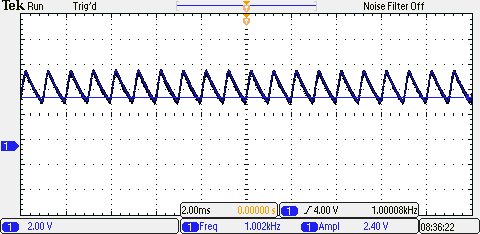
\includegraphics[width=220pt]{figure/relax_osc_beforeboost.png}
\caption{1kHz signal generated by the relaxation oscillator.}
\label{relax_osc_b4boost}
\end{figure}
\par Although the output voltage is suppose to switch from positive to negative $V_cc$, we found that the output voltage was only around 1.6V, which was below the turn on voltage of the LED. We tried using the signal as a switch with an additional 5V with a resistor to ``boost up" the signal to the LED, but had trouble figuring out how to arrange the activation signal with respect to the output LED and the rest of the circuit the for this purpose. By building an amplifier connecting to the output of the relaxation oscillator, we were able to attain a output voltage of around 3V while retaining the 1kHz signal.
\par When soldered together, this circuit served as a convenient module that can be easily moved to change the light incident on the detector, without the bulkiness of the waveform generator.
\subsection{Simulation}
d)              Multisim circuits, if any.

e)               If appropriate, a description of the theory behind your experiment.
\section{Experiment and Results}
f)                A description of the experiments you performed with your circuit and the measurements you made, including your experimental methods, your raw data (in tabular or graphical form), and data and error analysis.
Since some of our component did not come with spec sheets We conducted initial measurements to get a sense of what the 
\subsection{Calibrating Phototransistors}
\par Initially, we used a photoresistor to detect our optical signal. Even though the photoresistor gave a sufficiently large range (267$\Omega$ to 4.353k$\Omega$) of continuous signal change, there was significant lag between the circuit signal response shown on the oscilloscope relative to when we actuated the change. 
\par We improved the performance of the detection module by using the OP802SL NPN phototransistor, as this resolves the lagging issue seen with the phototransistors. We had a lot of difficulty in testing whether the phototransistor gave a response, so we began by first building a test circuit where we attached a 12V power supply to the collector and the --- giving a response.  We chose to use a red LED because its wavelength is closer to the peak on the spectral response graph as detailed in the OP802SL spec sheet.Since the light incident on the detector is what changes the signal through the base, the base should be connected to nothing, as denoted in most schematics on phototransistor spec sheets\footnote{In fact most manufacturer sells two-pronged, phototransistors without the base.}
\par  continuous instantaneous circuit response,
Approx linear response as expected since inside operating region, use for calibrating theremin. 
\begin{figure}[h!]
 \centering
 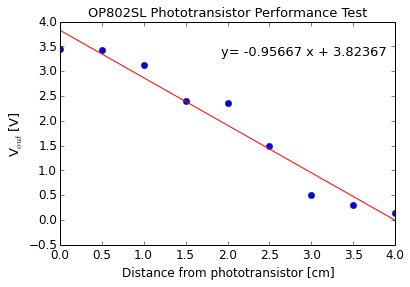
\includegraphics[width=220pt]{figure/phototransistor_performance}
\caption{Quantify the performance of the phototransistor by varying its separation distance from a red (660nm), 1kHz, 4V$_{Vpp}$ LED source.}
\label{phototransistor_performance}
\end{figure}
\section{Conclusion}
g)              Conclusions.

Possible future improvements -----etcs
\section*{Acknowledgments}
\begin{footnotesize}
The author would like to acknowledge support from the GSI and Professor Holzapfel in this lab in addressing our questions about how the circuits work, assisting us with the initial circuit design, and suggesting ways to improve its performance.  We also appreciate helpful discussion and debugging assistance from Elijah Campbell's group that helped this work.
\end{footnotesize}
  \section*{References}
 \begin{footnotesize}
\begin{enumerate}[label={[\arabic*]}]
\setlength\itemsep{0.001em}
 \item Horowitz, Paul, and Winfield Hill. \textit{The Art of Electronics}. Cambridge: Cambridge UP, 1989. Print.
 \item ``Lab 5 - JFET Circuits II. " \textit{Donald A. Glaser Advanced Lab.} Regents of the University of California, n.d. Web. 01 May. 2015.
 \item Nichole. "Create a DC Power Supply." \textit{Instructable}. N.p., n.d. Web. 1 May 2015.
  \item `` Lab 8 - Op Amps III " \textit{Donald A. Glaser Advanced Lab.} Regents of the University of California, n.d. Web. 07 May. 2015.
  \item ``Lab 12 - Final Project " \textit{Donald A. Glaser Advanced Lab.} Regents of the University of California, n.d. Web. 07 May. 2015.
 \item "Op-amp Relaxation Oscillator." \textit{Electronic and Electric Circuit Simulation.} N.p., n.d. Web. 9 May 2015.
 \item Eisenman, Bonnie. "Illumaphone: Light-based Musical Instrument with Arduino." \textit{Instructables}. N.p., n.d. Web. 10 May 2015.
\end{enumerate}
  \end{footnotesize}
\end{document}
%\subsubsection{Photoresistor Calibration}
%\begin{table}
%    \begin{tabular}{l|l}
%                                 & Resistance [$\Omega$] \\ \hline
%	Dark                          & 4.353k     \\ \hline
%    Ambient Light                 & 1.205k     \\ \hline
%    RED LED (3V)  & 267.3      \\ 
%    \end{tabular}
%    \label{photor}
%    \caption{Photoresistor resistance range for different light setting.}
%\end{table}